
\chapter{Background}
\label{chap:background}

\epigraph{"Today, CAN has established itself worldwide as the backbone for the networking of embedded systems, and this not only in automotive technology"}{Dr. Siegfried Dais, Prof. Dr. Uwe Kiencke, Martin Litschel}

\section{Intra Vehicle Networks}
\label{sec:vni}
Today's automobiles contain a series of different electronic components networked together to be responsible for monitoring and controlling the state of the vehicle. Each component can communicate with all other components on the same sub-network. The safety of the vehicle relies on near real time communication between these various ECUs. While communicating with each other, ECU's are responsible for predicting crashes, detecting skids, performing anti-lock braking (ABS), etc. \cite{Yadav16}. There are only a couple of operations that are performed without using computer control (with the parking brake and steering being the last holdouts) \cite{Kosher}. 

\subsection{Sub-Networks}
In most real architectures a series of domains are defined that correspond to different features of the car, often corresponding to dedicated sub-networks (i.e. Powertrain Control Module) within a single vehicle. The European Union Agency For Network And Information Security (ENISA) distinguishes between 6 different domains\cite{Enisa}, as is illustrated in figure \ref{fig:enisa}. These are:
\begin{itemize}
	\item \textbf{Powertrain Control Module (PCM):} Consists of engine control Units that control a set of actuators on the internal combustion engine, as well as transmission control units that change the gears to ensure optimal engine performance. 
	
	\item \textbf{Chassis Control:} Ensures control of the vehicle with regard to it's surroundings (e.g. steering, airbag, braking, etc.)
	
	\item \textbf{Body Control:} Compromises all ECU's that perform functions within the context of the passenger's compartment and/or trunk (e.g. dashboard, doors, windows and seatbelt, etc.).
	
	\item \textbf{Infotainment Control:} This domain includes navigational services (i.e. GPS), communications (i.e. Cellular) and entertainment (i.e. Radio).
	
	\item \textbf{Communications Control:} Unlike all previous modules this one does not compromise a single sub-network but rather a series of communication features offered by a telematics control unit (e.g. Wifi).
	
	\item \textbf{Diagnostic and Maintenance systems} This concerns all the various diagnostics and maintenance solutions that can be connected to the OBD-II port.
\end{itemize}

\begin{figure}[h]
	\label{fig:enisa}
	\centering
	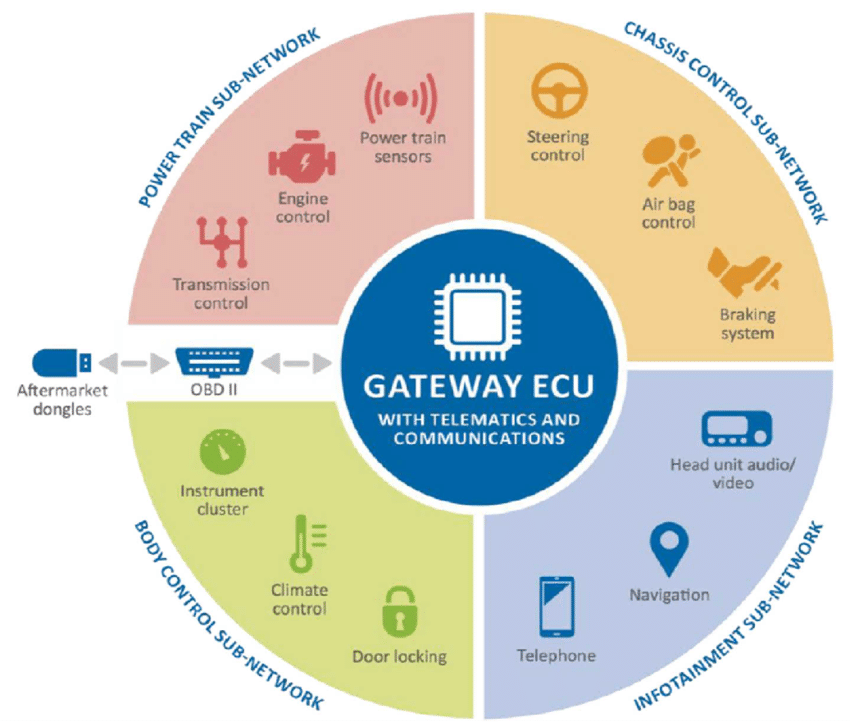
\includegraphics[width=\textwidth]{enisa.png}
	\caption{Typical intra vehicle network infrastructure \cite{Enisa}}
\end{figure}

On top of their functional differences, these sub-networks often implement different network communications protocols. This means that there are multiple communication standards that are employed even within a single vehicle. The most common ones are: Controller Area Network (CAN), Local Interconnect Network (LIN), Media Oriented Systems Transport (MOST), FlexRay and LVDS\cite{Tuhoy}. Each of these protocols specifies how messages are exchanged within the appropriate sub-network and are chosen to best service the needs of a specific domain, as is illustrated in figure \ref{fig:network_technologies2} and \ref{fig:network_technologies}.

\begin{figure}[h]
	\label{fig:network_technologies2}
	\centering
	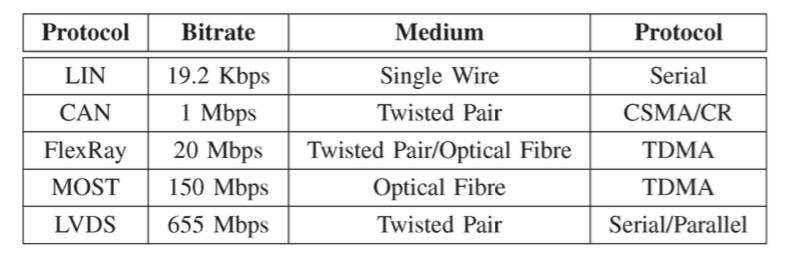
\includegraphics[width=\textwidth]{network_technologies2.png}
	\caption{An overview of different network technologies and their characteristics \cite{Tuhoy}.}
\end{figure}

\begin{figure}[h]
	\label{fig:network_technologies}
	\centering
	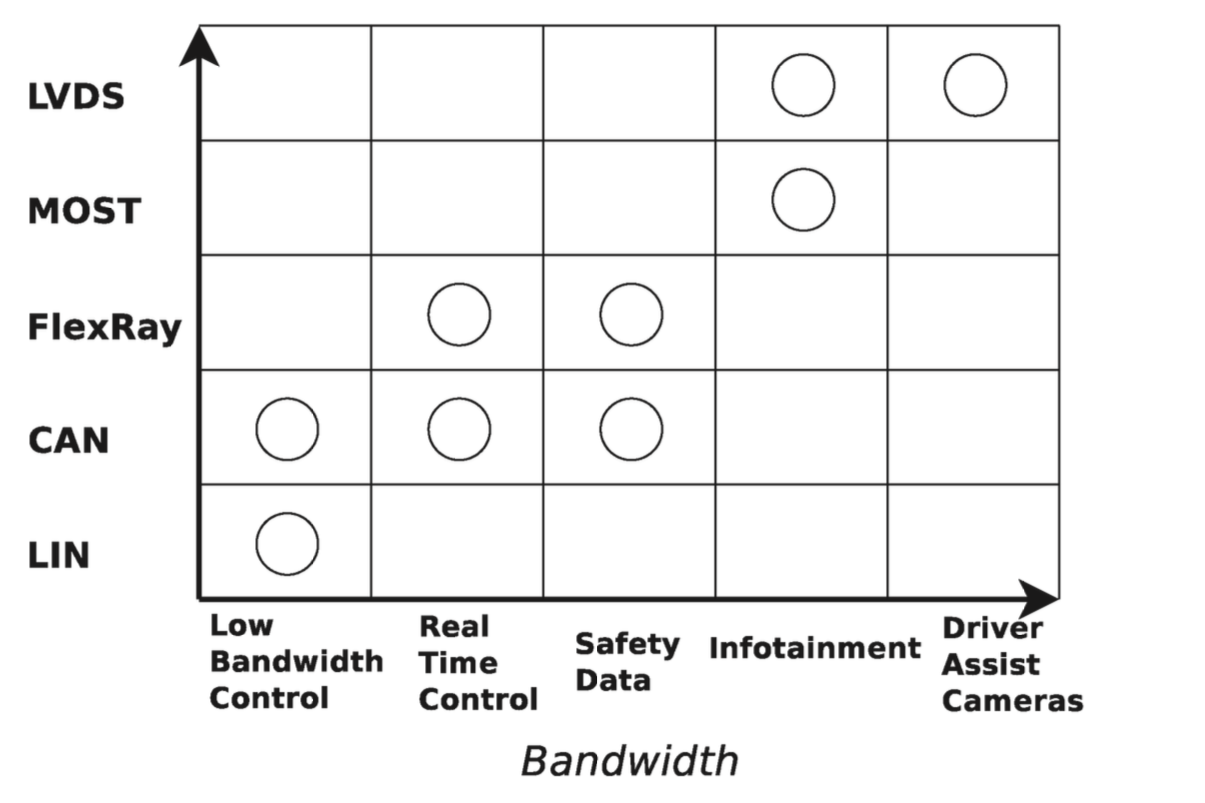
\includegraphics[width=\textwidth]{network_technologies.png}
	\caption{Mapping of traffic types to network technologies \cite{Tuhoy}.}
\end{figure}

A critical component in these types of networks (the presence of sub-networks with different communication protocols) is the Gateway ECU. This component performs a frame or signal mapping function between two communication systems, thereby allowing ECU's on different sub-networks using distinct communication protocols to exchange messages nonetheless. 
On top of acting as an intermediate between the different sub-networks of the vehicle, the Gateway also acts as an entry point for OBD-II messages. Any message sent via the OBD-II DLC will be translated and forwarded by the Gateway to the appropriate sub-network. It comes as no surprise that this component will play a crucial role when introducing access control to the OBD-II interface.

\subsection{Example: ABS}
Let's take a closer look at ABS to get a sense of how the intra vehicle network operates. ABS was designed to keep the wheels from locking up during braking. It consists of 3 main components: wheel speed sensors, a pump and a controller. Here's how it works\cite{wiki:ABS}:

\begin{itemize}
	\item The controller monitors the wheel speed sensors constantly (So each speed sensor periodically sends a message to the Controller).
	
	\item The controller will recognize a wheel locking whenever it detects a rapid deceleration.
	
	\item Whenever it does detect a wheel locking up, it will use the pump (again by sending a message over the network) to regulate the pressure on the brake of that particular wheel, thereby keeping it from locking up.
\end{itemize}

\section{CAN}
\label{sec:can}

The CAN protocol has become a ubiquitous part of the automotive industry. In the context of internal vehicle networks, CAN messages have multiple purposes: First, there are informative messages that are designed to transmit data from and to ECU's (e.g. the Anti-Lock System (ABS) broadcasting the speed of each wheel). Second, there are action messages that are designed to request another ECU to perform an action (e.g. adaptive Cruise Control (ACC) module requesting the brakes to be applied). Third, there are the diagnostic messages defined by the OBD-II protocol. \cite{MillerB} Naturally the last type of message is the focus of this paper. The following paragraphs are dedicated to the CAN protocol.

\subsection{Brief History} 
\label{subsec:can:briefhistory}

The history of CAN starts in 1983 when a couple of engineers at Bosch (soon aided by engineers from Mercedes-Benz and Intel) start developing a new serial bus system for use in the automobile industry. It wasn't long before CAN was officially introduced at the SAE congress in Detroit as: 'Automotive Serial Controller Area Network'. The main characteristics of this protocol were: 

\begin{itemize}
	\item An arbitration method that allows bus access to the message with the highest priority without delays.
	\item No master CAN node that is in charge of the bus.
	\item Transmitted messages are identified by their content, not by their destination or origin.
	\item This identification also determines the priority of the message within the network.
\end{itemize}

It didn't take long before the first CAN controller chips were developed in 1987 (by Intel and Philips respectively) and the first official CAN specifications were standardised in the 90's, effectively paving the way for the CAN protocol to become an industry staple as it is today. To this day Bosh has been making sure that all CAN chips comply with their proposed standards in order to avoid incompatible implementations. \footnote{For a comprehensive history of the CAN protocol confer \cite{CANhistory}}.

\subsection{Architecture}
\label{subsec:can:architecture}

A typical CAN network consists of a series of nodes (with a minimal of 2 in order for the network to be functional) connected by a two-wire bus. It is important to note that there are 2 physical CAN specifications: high speed CAN (see \cite{ISO11898-2}) and low speed (or fault tolerant) CAN (see \cite{ISO11898-3}). Every CAN node consists of:
\begin{itemize}
	\item CPU: effectively the 'brain' of the node, deciding what messages are sent and taking the appropriate course of action whenever a message is received.
	\item Controller: in charge of reading and writing bits to and from the CAN bus.
	\item Transceiver: acts as in an intermediate between the bus and the controller, thereby translating between different signal levels.
\end{itemize}

This architecture specifies the minimum requirements of a CAN node. More often than not these nodes will include other components (e.g. sensors, actuators) that are connected to the CPU. It should be clear from this specification that this architecture applies to any common vehicle network (e.g. ECU's act as CAN nodes).

\subsection{CAN Frames}
\label{subsec:can:frames}

Since CAN is a message based protocol, it facilitates communication by transmitting short bursts of data called CAN frames. There are four different types of CAN frames:
\begin{itemize}
	\item Data frame: used to transmit data with a specific identifier.
	\item Remote frame: used to request the transmission of data with a specific identifier.
	\item Error frame: transmitted whenever a node detects an error on the bus.
	\item Overload frame: transmitted by a node to include a delay between data or remote frame.
\end{itemize}

There are 2 frame formats: base frame format and the extended frame format. The only difference being that the extended frame format uses a 29 identifier bits and the base frame format only uses 11. Table \ref{table:1} lists all the fields of a base format data frame. The extended frame format is the same except for an additional identifier field (18 bits) right after the identifier extension bit (IDE) field.

\begin{table}[]
	\begin{tabular}{|l|l|l|}
		\hline
		\rowcolor[HTML]{9B9B9B} 
		name & size (bits) & purpose \\ \hline
		start-of-frame & 1 & Denote start of transmission \\ \hline
		identifier (ID) & 11 & Unique identifier + determines priority \\ \hline
		remote transmission request (RTR) & 1 & must be 1 for remote frames \\ \hline
		identifier extension bit (IDE) & 1 & must be 1 for extended frames \\ \hline
		reserved bit & 1 & reserved for future use \\ \hline
		data length code (DLC) & 4 & length of data field \\ \hline
		data field & 64 & data to be transmitted \\ \hline
		cyclic redundancy check (CLC) & 15 & check for errors \footnotemark  \\ \hline
		CRC delimiter & 1 &  must be 1 \\ \hline
		acknowledgement slot (ACK) & 1 & used for message acknowledgement \\ \hline
		ACK delimiter & 1 & must be 1 \\ \hline
		end-of-frame (EOF) & 7 & must be 1  \\ \hline
	\end{tabular}
	\caption{base frame format \cite{wiki:CAN}}
	\label{table:1}
\end{table}

\footnotetext{A cyclic redundancy check is a way of detecting accidental changes to transmitted data (e.g. due to noise, interference, etc). For more information on cyclic redundancy checking see \cite{wiki:CRC}.}

\subsection{Data Transmission}
\label{subsec:can:data_transmission}

The operation of the CAN protocol is pretty straightforward: a node transmits a message with a specific ID on the bus. Any node that is connected to the same bus is able to receive the message (broadcast), but only the nodes that are listening for this specific ID will take action. It is worth noting that the ID is used to identify the content, not the sender or receiver. As a matter of fact CAN does not provide any way of authenticating the sender or receiver, which results in various security related difficulties (see \ref{sec:issues}) . Aside from identifying the content, this ID is also used to solve the issue of message arbitration. CAN is a carrier sense multiple access protocol, whereby each nodes observes the bus before transmitting data on it, if it detects that the bus is in use it waits for some time before trying again. This does not prevent nodes from starting a data transfer at the same time, this is where bit wise message arbitration provides a solution. \cite{CANarbitration}.

\subsection{Message Arbitration}
\label{subsec:can:message_arbitration}

Whenever 2 (or more) nodes initiate a transmission on the bus at the same time, bit wise message arbitration is performed. Every bit of the message ID can be either 1 or 0. The CAN specifications use the term dominant (logical 0) and recessive (logical 1). These terms originate from the fact that whenever more than one bit is simultaneously written to the bus, and one of these is dominant, the dominant bit 'wins', meaning a logical 0 will be seen on the bus. Whenever a node transmits a logical 1 but sees a logical 0, it realizes that there is a contention and re-queues its message for later transmission. Since the identifier is transmitted at the start of the CAN frame, the node with the numerically lowest identifier transmits more zeros at the start of the frame, and that is the node that wins the arbitration. Concisely put we can say that messages with lower ID's have priority over messages with higher ID's. The decision to identify messages by their content (instead of their sender or receiver) is motivated by the fact that certain very important types of messages (e.g. errors) can be given a very low id, thereby ensuring they are less prone to be delayed. This approach does introduce some issues when it comes to security (see \ref{sec:issues}).

\subsection{Layering}
\label{subsec:can:layering}

In line with most networking protocols, it is common practice to decompose them into different abstract layers. This is done to simplify the design and make modularisation easier \cite{wiki:ProtocolStack}. In the case of CAN the layers are:

\begin{itemize}
	\item \textbf{Application layer:} OBD-II, CANOpen, VulCAN etc.
	\item \textbf{Object layer:} message filtering and status handling.
	\item \textbf{Transfer layer:} error detection, message arbitration, bit timing, etc.
	\item \textbf{Physical layer:} signal voltages, pin-out configuration, etc.
\end{itemize}

\subsection{Security Issues}
\label{subsec:can:security_issues}

The CAN protocol has a number of inherent vulnerabilities that are common to any implementation. The most obvious and important ones are:

\begin{itemize}
	\item \textbf{Broadcast nature:} CAN frames are both physically and logically (no destination address) broadcasted on the network. This means that a malicious node on the bus can snoop on all communications or even worse: send packets to any other node on the network \cite{Kosher}. 
	
	\item \textbf{No authentication:} CAN frames do not have source identifier fields, so there is no way for any node to be aware of the source of any messages it receives. This means that any compromised component (or any other form of unsanctioned access to the CAN bus for that matter) can inject arbitrary messages. Whereas the system has no way of knowing these messages were not sent by the appropriate component \cite{Kosher}\cite{CANissues}.
	
	\item \textbf{No encryption:} We've mentioned that speed and timing are deemed more important to the safety and performance of the vehicle than data security. A clear result of this is the decision to omit any encryption capabilities. This is because the limited  computational power of ECU's makes it difficult to implement robust cryptographic algorithms. \cite{CANissues}.  
	
	\item \textbf{Susceptibility to Denial of Service (DoS):} This problem arises mainly from the protocol's message arbitration method. Any malicious node can effectively spam the bus with high priority messages (only zeroes as ID) causing all other nodes to back off (no protection against "babbling idiots"\cite{Pike15})\cite{Kosher}.
	
	\item \textbf{Not Byzantine fault tolerant:} In most distributed systems, malicious attacks and software errors can cause a node to exhibit Byzantine (i.e. arbitrary) behaviour\cite{Byzantine}. Because of the distributed nature of any CAN system, there is imperfect information on whether a component has failed (or has been compromised by attack) or not. This could result in situations where entire system services fail since a common consensus cannot be reached\cite{wiki:ByzantineFault}. \footnote{For more information on Byzantine faults, and how it is tolerated in a system see \cite{Byzantine} and \cite{wiki:ByzantineFault}.}.
	
\end{itemize}

For more information on the CAN protocol see \cite{ISO11898-2} and \cite{ISO11898-3}.

\section{OBD-II}
\label{sec:obd}

\subsection{Design Goals} 
\label{subsec:obd:design_goal}

OBD-II (On Board Diagnostics) is a specification that was introduced to allow for self diagnostic and reporting functionality for ECU's inside a vehicle, and has been mandatory in every car produced in the united states since 1996. \cite{wiki:OBD}. It allows users (testers, developers, repairmen, etc) to query ECU's about diagnostics information in order to perform a detailed analysis of the vehicles internal systems. Specifically the goals of OBD-II upon introduction were: 
\begin{itemize}
	\item Standardisation: information is communicated in a standardized format to allow for 1 tool to be used on many vehicles.
	\item Certification: Every vehicle manufacturer required to submit certification application for review and approval, which includes a detailed description of how the OBD-II protocol was implemented.
	\item Help lowering emissions by identifying emission controls in need of repair.
\end{itemize} 
The system can also be very useful in a number of other situations: A repairman looking for a specific component that is to be repaired, an employee at the factory testing all components before the vehicle is ready to be sold, a policeman analysing a vehicle after a crash to determine what caused the accident, a software developer testing the operation of a newly developed ECU, etc. 
\newline

\subsection{Brief History}
\label{subsec:obd:brief_history} 

There were a lot of different proprietary diagnostics systems introduced over the years, before a standard arrived with the introduction of OBD-II. This brief history cited from \cite{OBDhistory} does a decent job of concisely explaining how OBD-II came to be:

\begin{displayquote}
	The origins of OBD-II actually date back to 1982 in California, when the California Air Resources Board (ARB) began developing regulations that would require all vehicles sold in that state starting in 1988 to have an onboard diagnostic system to detect emission failures. The original onboard diagnostic system (which has since become known as OBD-I) was relatively simple and only monitored the oxygen sensor, exhaust gas circulation system, fuel delivery system and engine control module.
	
	OBD-I was a step in the right direction, but lacked any requirement for standardization between different makes and models of vehicles. You still had to have different adapters to work on different vehicles, and some systems could only be accessed with costly "dealer" scan tools. So when ARB set about to develop standards for the current OBDII system, standardization was a priority: a standardized 16-pin data link connector (DLC) with specific pins assigned specific functions, standardized electronic protocols, standardized diagnostic trouble codes (DTCs), and standardized terminology.
	
	Another limitation of OBD-I was that it couldn't detect certain kinds of problems such as a dead catalytic converter or one that had been removed. Nor could it detect ignition misfires or evaporative emission problems. Furthermore, OBD-I systems would only illuminate the MIL light after a failure had occurred. It had no way of monitoring progressive deterioration of emissions-related components. So it became apparent that a more sophisticated system would be required. The California Air Resources Board eventually developed standards for the next generation OBD system, which were proposed in 1989 and became known as OBD-II. The new standards required a phase-in starting in 1994. The auto makers were given until the 1996 model year to complete the phase-in for their California vehicles.
	
	Similar standards were incorporated into the federal Clean Air Act in 1990 which also required all 49-state vehicles to be OBD-II equipped by 1996 -- with one loophole. The OBD-II systems would not have to be fully compliant until 1999. So some 1996 OBD-II systems may lack one of the features normally required to meet the OBD-II specs, such as the evaporative emissions purge test.
\end{displayquote}

\subsection{DLC}
\label{subsec:obd:dlc}

In order to allow a user to communicate with the vehicle's internal network, OBD-II introduces the data link connector (DLC). The DLC is a 16-pin hardware interface (although only 9 pins are specified by the standard) that is generally found close to the steering wheel (by law it is required to be installed within 0.61 m of the steering wheel) \cite{wiki:OBD}. There are 2 basic types of connectors: Type A as seen in figure \ref{fig:typeA} (using a 12V power supply) and Type B as seen in figure \ref{fig:typeB} (using a 24V power supply). the design of the two connector types prevents the insertion of a type A male plug into a type B female socket.

\begin{figure}[h]
	\label{fig:typeA}
	\centering
	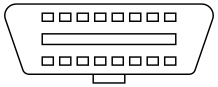
\includegraphics{typeA.png}
	\caption{Type A female connector \cite{wiki:OBD}}
\end{figure}

\begin{figure}[h]
	\label{fig:typeB}
	\centering
	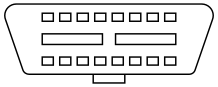
\includegraphics{typeB.png}
	\caption{Type B female connector \cite{wiki:OBD}}
\end{figure}

\subsection{PID's}
\label{subsec:obd:pid}

OBD-II introduces parameter PID's, which are codes used to identify and query specific data. The protocol is designed to work with multiple signalling protocols (the messaging protocol that is used to request and receive data from the network) but the CAN protocol is mostly implemented (Since 2008 all new vehicles sold in the us implement this signalling protocol\cite{OBDconnector}). \newline
\newline
There are multiple ways for a user to interact with this interface:
\begin{itemize}
	\item Standard Diagnostic scanning tool: a dedicated device that consists of a small hand-held module (equipped with a small screen and some buttons) connected to a male DLC-connector (The DLC inside the vehicle is always female).
	
	\item An advanced Diagnostic scanning tool that includes a DLC-connector with wifi/Bluetooth compatibility, allowing for remote diagnostics using a smartphone.
	
	\item A DLC-connector with a usb adapter allowing access via dedicated software on a pc. Since 2014 all new cars in the US support the SAE J2534 "PassThru" standard, which is a Windows API (Application Programming Interface) that provides a standard way to communicate with a car's internal buses \cite{Kosher}.\footnote{For more information on SAE J2534, see the full API reference at: https://tunertools.com/prodimages/DrewTech/Manuals/PassThru\textunderscore API-1.pdf}
	
	\item A data logger, which is designed to capture real-time data while the vehicle is in operation.
\end{itemize}

Typically the ODB-II is used like this (CAN as signalling protocol): First, the user enters the PID of the data he/she wants to query into a diagnostic tool. Second, this data is packaged in a CAN frame and sent on the CAN-bus. Third, the ECU that is responsible for the data identified by the PID in the message recognizes it as it's own, and transmits a CAN frame containing the requested data. Fourth, the diagnostic tool recognizes the response and displays the data to the user \cite{wiki:PID}. Aside from this, the OBD-II port can then be used to upgrade the ECU's firmware or to perform a myriad of diagnostic tasks.

\subsection{Security Issues}
\label{subsec:obd:security_issues}

It is a well-known fact that the automotive industry has always considered safety a critical engineering concern (especially since the public awareness around lethal accidents has only increased over the years). Unfortunately it is unclear whether developers (especially concerning the internal network) have considered the security in their design. However it seems this is not the case because of three reasons. First, there is no inherent support for addressing, encryption or authentication \cite{MillerB}. Second, most of the networks and ECU's were designed when access to the bus required physical access to the vehicle, therefore security was not a primary concern. Third, speed and timing are deemed more important to the safety and performance of the vehicle than data security \cite{Klinedinst05}. This vulnerability is worsened by the fact that the attack surface for modern automobiles is growing swiftly as more sophisticated services and communications features are incorporated into vehicles \cite{Kosher}. The OBD-II specification is one of these since the interface it introduces provides direct access to the internal vehicle network. This allows malicious agents to easily construct and insert CAN messages to alter the vehicle's behaviour, as has been frequently demonstrated by Charlie Miller and Chris Valasek's exploits \cite{MillerA}\cite{MillerB}\cite{MillerC}. Before analysing the attack vectors that OBD-II introduces, and the possible impact thereof on the safety and security of the vehicle, let's first take a closer look at CAN's shortcomings when it comes to safety.

